\chapter{Анализ предметной области}
\label{cha:analysis}

\section{Фотокамера}

Фотокамера (фотоаппарат) --- это прибор для получения на фотографическом материале действительного изображения предмета при фотографировании.~\cite{gost}

Цифровой фотоаппарат --- фотоаппарат, в котором для регистрации изображения используется фотоэлектрический принцип. В данной научно-исследовательской работе рассматривается этот тип фотоаппаратов в виду их повсеместного использования и универсальности. 

На рисунке 1.1 представлены основные элементы цифрового фотоаппарата.

\begin{figure}[!h]
	\center{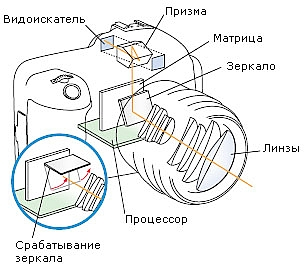
\includegraphics[scale=0.8]{assets/camera}}
	\caption{Основные элементы цифрового фотоаппарата}
\end{figure}

Кратко принцип работы цифрового фотоаппарата можно описать следующим образом: фотон попадает на светочувствительную матрицу, световая энергия преобразуется в электрическую, которая посредством дискретизации и квантования напряжения преобразует энергию в цифровые данные, которые в дальнейшем хранятся в памяти некоторой вычислительной машины с энергонезависимым запоминающим устройством.

В рамках данной работы наибольший интерес представляет фотоматрица --- специализированная аналоговая или цифро-аналоговая интегральная микросхема, состоящая из светочувствительных элементов (фотосенсоров). Матрица предназначена для преобразования спроецированного на нее оптического изображения в аналоговый сигнал (или в набор цифровых данных, если в матрице присутствует аналого-цифровой преобразователь).

\section{Цифровое изображение}

Изображение, получаемое фотокамерой, можно определить как двумерную функцию $f(x,\;y)$, где $x$ и $y$ --- пространственные координаты. Значение функции $f$ в некоторой точке, задаваемой парой координат $(x,\;y)$, является положительной скалярной величиной, называемой интенсивностью, или яркостью изображения в этой точке.~\cite{gonsales}

Для изображений, получаемых \textit{цифровой} фотокамерой, величины $x, y$ и $f$ принимают конечное число дискретных значений. Такие изображения называются цифровыми.

Модель процесса получения дефокусированного цифрового изображения в пространственной области может быть представлена в виде выражения~(1.1)~\cite{defocus_model}:

\begin{equation}
	g(x,\;y) = f(x,\;y) \oplus h(x,\;y) + \eta(x,\;y),
\end{equation}

где: 

\begin{itemize}
	\item $f(x,\;y)$ --- функция, описывающая исходное изображение (неискаженное);
	\item $g(x,\;y)$ --- функция, описывающее дефокусированное изображение (искаженное);
	\item $h(x,\;y)$ --- функция размытия точки (или оптическая передаточная функция), или ядро искажающего оператора \cite{frt};
	\item $\eta(x,\;y)$ --- функция шума;
	\item символ <<$\oplus$>> --- оператор свертки.
\end{itemize}

Задача восстановления изображения заключается в поиске наилучшего приближения $\hat{f}(x,\;y)$ исходного изображения.

\subsection*{Cвертка (конволюция)}

Применительно к обработке цифровых изображений операция свертки может быть интерпретирована следующим образом: на основе некоторого множества пикселей в исходном изображении вычисляется новый пиксель результирующего (искаженного ядром свертки) изображения.

На рисунке 1.4 представлен пример выполнения операции свертки. Для вычисления новых значений используется т.~н. ядро свертки: на приведенном рисунке ядром является матрица зеленого цвета размером $3\times3$.

%В общем случае применение операции свертки к изображению приводит к уменьшению его размера.

\begin{figure}[!h]
	\center{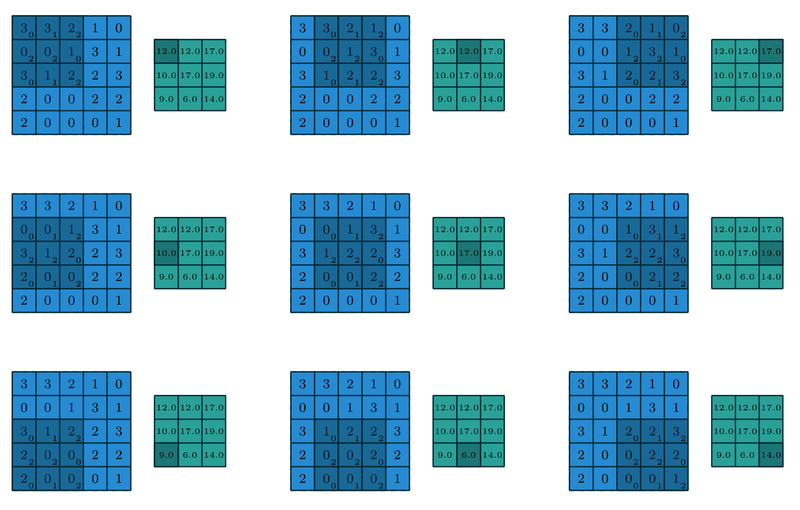
\includegraphics[scale=1.5]{assets/convolution_example}}
	\caption{Пример выполнения операции свертки}
\end{figure}

В зависимости от выбранного ядра свертки, примененного к изображению, можно получить тот или иной эффект: размытость, повышение резкости, обнаружение контуров, граничное обнаружение и др.

Математически операцию двумерной свертки изображения в пространственной области можно описать в виде выражения (1.2).

\begin{equation}
	f(x,\;y) \oplus h(x,\;y) = \sum_{i = -a}^{a} \sum_{j = -b}^{b} f(x + i, y + j) \cdot h(x,\;y),
\end{equation}

где $a = \cfrac{M-1}{2}, b = \cfrac{N-1}{2}$, M, N - размеры изображения,.

Получение функций $f(x,\;y)$ и $h(x,\;y)$ из выражения (1.2) путем выполнения обратных действий приводит к получению большой системы уравнений, решение которой является нетривиальной и трудоемкой задачей.~\cite{teorema} Упростить ее решение может \textit{теорема о свертке}, согласно которой операция свертки в пространственной области эквивалентна поэлементному умножению в частотной области:

\begin{equation}
	f(x,\;y) \oplus h(x,\;y) \longleftrightarrow F(u,\;v) \cdot H(u,\;v),
\end{equation}

где $F(u,\;v)$, $H(u,\;v)$ - Фурье~--~образы (спектры) функций $f(x,\;y)$ и $h(x,\;y)$ соответственно.

Преобразование Фурье некоторой функции $f(x)$ определяется выражением (1.4):

\begin{equation}
	F(\omega) = \frac{1}{\sqrt{2\pi}} \cdot \int_{-\infty}^{+\infty}f(x) \cdot e^{-i\cdot x \cdot \omega}~dx.
\end{equation}

Преобразование Фурье позволяет разложить исходный цифровой сигнал на гармонические (частотные) составляющие, что потребуется для выделения шумов.

\clearpage

\section{Причины дефокусировки фотокамеры}

На рисунке 1.3 приведена иллюстрация, поясняющая физический принцип получения расфокусированного изображения.~\cite{graphic}

\begin{figure}[!h]
	\center{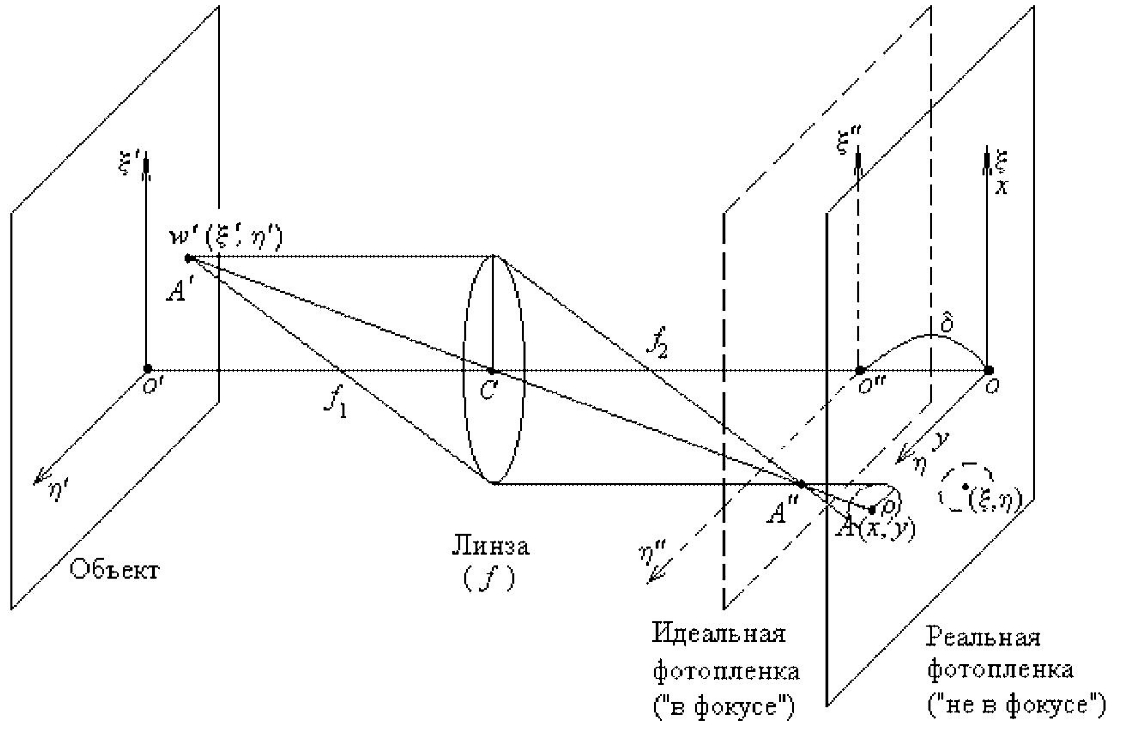
\includegraphics[scale=0.5]{assets/schema}}
	\caption{Принцип получения расфокусированного изображения}
\end{figure}

Пусть снимаемый объект, полагаемый плоским из-за его удаленности, и фотопленка (или матрица сенсоров) расположены параллельно тонкой линзе по разные стороны от нее. 

Пусть $f_1$ --- расстояние от линзы до объекта, а $f_2$ --- расстояние от линзы до фотопленки (матрицы), установленной в <<фокусе>>, а $\sigma$ --- погрешность фокусировки изображения. Таким образом, реальная фотопленка установлена <<не в фокусе>>.

Как видно из рисунка, лучи из точки $A'$ после их прохождения через линзу отобразятся на реальной фотопленке не в точку, а в некоторое размытое пятно, определяемое т.~н. функцией размытия точки, или функцией искажения ядра.~\cite{schema2}

%Соответственно при использовании фотоаппарата изображение будет расфокусированным, если неправильно настроен фокус камеры.

\clearpage

\section*{Вывод}

Для получения восстановленного изображения необходимо произвести обратные вычисления, однако деконволюция (операция, обратная свертке) математически очень трудоемкая и нетривиальная операция. Вследствие этого были разработаны методы восстановления, решающие поставленную задачу иными способами.